\documentclass{beamer}


% \usepackage{CJKnumb}\usepackage{beamerthemesplit}

\mode<article>
{
  \usepackage{beamerbasearticle}
  \usepackage{fullpage}
  \usepackage{hyperref}
}

%\usepackage{beamerthemesplit} 
%\usepackage{beamerthemeshadow}  
%\usepackage[width=2cm,dark,tab]{beamerthemesidebar}


% Setup appearance:

%\usetheme{Darmstadt}
\usefonttheme[onlylarge]{structurebold}
\setbeamerfont*{frametitle}{size=\normalsize,series=\bfseries}
\setbeamertemplate{navigation symbols}{}


% Standard packages

\usepackage[english]{babel}
%\usepackage[latin1]{inputenc}

\usepackage{epsf}
\usepackage{amsmath,amssymb}
\usepackage{graphicx}
\usepackage{tabularx}

% \usepackage[usenames,dvipsnames]{color}
\newcommand{\redc}[1]{{\color{red} #1}}
\newcommand{\bluec}[1]{{\color{blue} #1}}
\definecolor{myyellow}{HTML}{FFB700}
\newcommand{\yellowc}[1]{{\color{myyellow} #1}}
\newcommand{\greenc}[1]{{\color{green} #1}}
\renewcommand{\v}[1]{\textbf{\textit{#1}}}
\renewcommand{\d}[1]{\textrm{#1}}


%\usetheme{Boadilla}
%\usetheme{Copenhagen}
%\usetheme{Madrid}
\usetheme{Singapore}


\begin{document}
%\title{Comparative atomistic and coarse-grained study of water: Simulation details vs. Simulation feasibility}
%\title[Optimizing SPME]{Optimizing Working Parameters of the Smooth Particle Mesh Ewald Algorithm}
\title[]{Parameter Optimization Methods for the Non-bonded Interactions}
%
\author{Han Wang}
\institute[SMS@PKU] {School of Mathematical Sciences, Peking University, Bejing\\
\vskip 0.4cm
Joint with: Florian Dommert, Christian Holm, Pingwen Zhang}
\date[THU Aug 2009]{Freie Universit\"at Berlin}
\frame{\titlepage}

\begin{frame}{Non-bonded interactions}
  In molecular dynamics simulations, the calculation of
  \redc{non-bonded interactions} is \redc{expensive}.
  \begin{align*}
    \bluec{U = U (\v r_1, \v r_2, \cdots, \v r_N)}.
  \end{align*}
  Only \redc{pairwise} interactions with \redc{periodic} boundary condition:
  \begin{align*}
    \bluec{U = \frac12\sum^\ast_{n}\sum_{i,j} U (\v r_{ij} + \v n)}.
  \end{align*}
  $\v r_{ij} = \v r_i - \v r_j$ and $\v n = n_1 \v a_1 + n_2 \v a_2 +
  n_3 \v a_3$ is the lattice in real space and the $\v a_\alpha, \
  \alpha=1,2,3$, are box vectors. \vfill
\end{frame}

\begin{frame}{Short-range and long range}
  % {Slow decay of the interaction with respect to distance}
  \vfill
  \begin{itemize}
  \item \redc{Short-range} interaction: Lennard-Jones
    \begin{align*}
      \bluec{
        U_{\textrm{LJ}}(\v r_{ij}) = 4\varepsilon
        \bigg[
        \Big(\frac{\sigma}{\vert \v r_{ij}\vert}\Big)^{12} -
        \redc{\Big(\frac{\sigma}{\vert \v r_{ij}\vert}\Big)^6}
        \bigg]
      }
    \end{align*}
  \item \redc{Long-range} interaction: electrostatic interaction
    \begin{align*}
      \bluec{
        U_{\textrm{ele}}(\v r_{ij}) =
        \frac{q_iq_j}{4\pi\varepsilon}
        \redc{\frac1{\vert \v r_{ij}\vert}}
      }
    \end{align*}
  \end{itemize}
  \vfill
  Different calculation methods: \redc{cut-off} method for short-range
  interactions and \redc{Ewald summation} for long-range interactions.
  \vfill
\end{frame}

\begin{frame}{Short range vs. long range}
  % {Slow decay of the interaction with respect to distance}
  \begin{figure}
    \centering 
    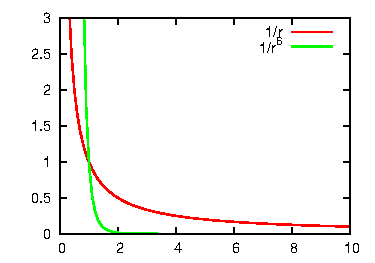
\includegraphics[width=0.8\textwidth]{figs/long-range/decay.pdf}
    \\{The function $\frac1r$ comparing with $\frac1{r^6}$. }
  \end{figure}
\end{frame}

\begin{frame}{Twin-range cut-off method for short-range interaction}
  \begin{figure}
    \centering 
    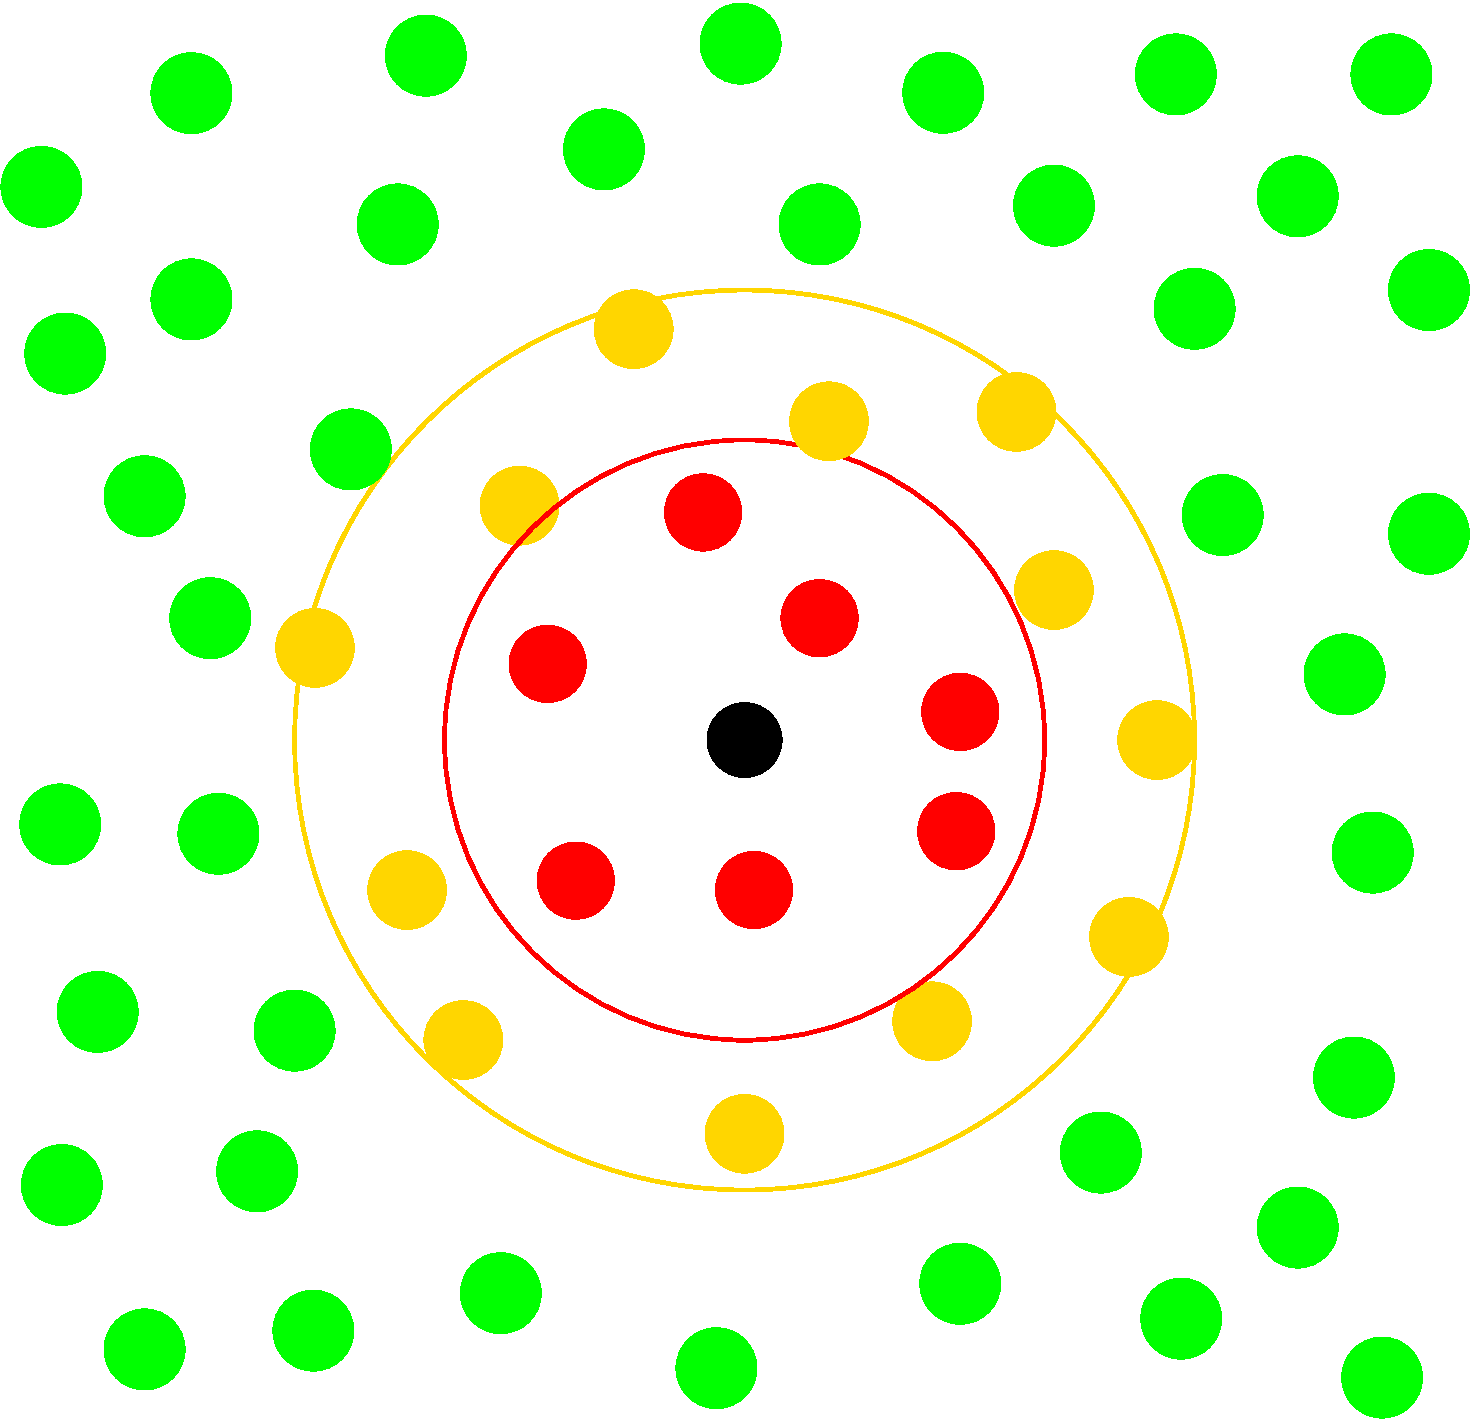
\includegraphics[width=0.5\textwidth]{figs/short-range//neighbor.pdf}
    \caption{Two cut-off radii: \redc{$r_1$} and \yellowc{$r_2$}.}
  \end{figure}
%   $r_1$, between $r_1$ and $r_2$, and
% out of $r_2$ by $\Omega_1^i$, $\Omega_2^i$ and $\Omega_3^i$, 
\end{frame}

\begin{frame}{Twin-range cut-off method}
  \vfill
  The neighbor particles are divided into three groups.
  \begin{itemize}
  \vfill
  \item \redc{Fall in $r_1$}: interactions are calculated every step.
  \vfill
  \item \yellowc{Between $r_1$ and $r_2$}: interactions are calculated every $M$
    steps. (When the neighbor list is updated)
  \vfill
  \item \greenc{Out of $r_2$}: interactions are neglected.
  \vfill
  \end{itemize}
\end{frame}

\begin{frame}{Error of the cut-off}
  The cut-off introduces error in the MD simulation.
  % Physical properties can be substantially affected by the cut-off radius.
  \begin{itemize}
  \item The phase diagram of Lennard-Jones fluid.
  \item Density profile of liquid-vapor interface.
  \item Surface tension.
  \item Free energy calculation.
  \end{itemize}
  \begin{figure}
    \centering
    \begin{minipage}[c]{.54\linewidth}
      \centering
      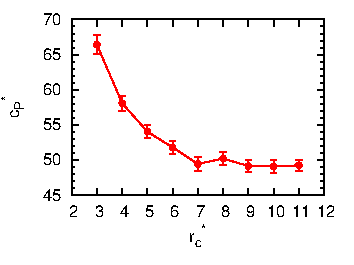
\includegraphics[width=1.\textwidth]{figs/short-range//natom-rcut-c.pdf}
    \end{minipage}
    \begin{minipage}[c]{.44\linewidth}
      \centering
      \caption{Constant pressure heat capacity $C_{\textrm{P}}^\ast$
        with respect to the cutoff radius $r_c^\ast$ at $T^\ast =
        1.36$ and $P^\ast = 0.1535$. }
    \end{minipage}
  \end{figure}
\end{frame}

\begin{frame}{The error of cut-off}
  We consider the root mean square (RMS) force error that is widely
  used in this field:
  \begin{align*}
   \bluec{\mathcal E(r_1, r_2, M) =
    \sqrt{\langle(\v F^{\textrm{exact}} - \v
      F^{\textrm{{approx}}})^2\rangle} }    
  \end{align*}

  The accumulated absolute displacement between two
  neighbor list updates is denoted by {$\v d_j$}.  \bluec{
  \begin{align*}
    \v F_i^{\textrm{exact}} & =
    \sum_{\redc{j\in\Omega_1^i}}\v F(\v r_{ij} + \v d_{ij}) +
    \sum_{\yellowc{j\in\Omega_2^i}}\v F(\v r_{ij} + \v d_{ij}) +
    \sum_{\greenc{j\in\Omega_3^i}}\v F(\v r_{ij} + \v d_{ij}),\\
    \v F_i^{\textrm{approx}} & =
    \sum_{\redc{j\in\Omega_1^i}}\v F(\v r_{ij} + \v d_{ij}) +
    \sum_{\yellowc{j\in\Omega_2^i}}\v F(\v r_{ij}).
  \end{align*}
  }
  Where {$\v d_{ij} = \v d_i - \v d_j$}.
\end{frame}

\begin{frame}[label=short-assumptions]{Assumptions}
  \vfill
  To
  calculate this error we need some assumptions:
  \begin{enumerate}
  \vfill
  \item $\v r_i,\ i=1,\cdots,N$ are random variables with \redc{uniform
    distributions} over the space.
  \item $\v d_i,\ i=1,\cdots,N$ are random variables having a \redc{normal
    distribution} with mean 0 and variance $d^2$, namely
    $\mathcal{N}(0, d^2)$.
  \item $\v r_i$ and $\v r_j$ are \redc{independent}, if $i\neq j$.
  \item $\v d_i$ and $\v d_j$ are \redc{independent}, if $i\neq j$.
  \item $\v r_i$ and $\v d_j$ are \redc{independent}, for any $i$ and $j$.
  \end{enumerate}
  \vfill
  \hfill\hyperlink{short-result-1}{\beamerreturnbutton{To Results}}
\end{frame}

\begin{frame}{The error estimate}
  \bluec{
  \begin{align*}
    \mathcal E^2 (\redc{r_1}, \redc{r_2}, \redc{M})
    = &
    (4\pi\rho)^2
    \redc{d}^2 \bigg\{
    \int_{\redc{r_1}}^{\infty}\frac13r^2U''(r)\d dr + 
    \int_{\redc{r_1}}^{\infty}\frac23rU'(r)\d dr 
    \bigg\}^2 +  \\
    &
    8\pi\rho\,
    \redc{d}^2 \bigg\{
    \int_{\redc{r_1}}^\infty\frac13\,[rU''(r)]^2\d dr + 
    \int_{\redc{r_1}}^\infty\frac23\,[U'(r)]^2\d dr  
    \bigg\} + \\
    &
    4\pi\rho\int_{\redc{r_2}}^\infty [rU'(r)]^2\d dr.
  \end{align*}
  }
  Where $\rho$ is the number density.
  The mean displacement $d$ can be related to the neighbor list
  updating frequency $M$ by
  \bluec{
    \begin{align*}\label{tmpeq:7}
      \redc{d} \approx \redc{M}\Delta t\sqrt{\frac{3k_BT}m},
    \end{align*}
  }
  Note: $\sqrt{\frac{3k_BT}m}$ is the mean velocity.
\end{frame}

\begin{frame}{The error estimate}
  The error estimate of the dispersion energy \bluec{$U(r) =-
    4\varepsilon(\sigma/r)^{m}$} is \bluec{
  \begin{align*}
    \mathcal E^2 (r_1, r_2, M)
    = \;&
    (\frac{16}3m\pi\rho\varepsilon\sigma^m)^2\redc{d}^2
    \bigg(\frac1{\redc{r_1}^{2m-2}}\bigg) +\\
    &
    2\frac{m^2+2m+3}{3(2m+1)}
    \pi\rho(8m\varepsilon\sigma^m)^2 \redc{d}^2
    \bigg(\frac1{\redc{r_1}^{2m+1}}\bigg) + \\
    &
    \frac{4}{2m-1}
    \pi\rho(4m\varepsilon\sigma^6)^2
    \bigg(\frac1{{\redc{r_2}}^{2m-1}}\bigg).
  \end{align*}
  }
\end{frame}

\begin{frame}
  \frametitle{Necessary conditions of parameter tuning}
  \vfill
  Parameter tuning:
  \vfill
  \begin{itemize}
  \item Given a \redc{predetermined accuracy}.
  \vfill
  \item Find the \redc{fastest} combination of working parameters\newline
    \redc{$r_1$, $r_2$} and \redc{$M$}.
  \end{itemize}
  \vfill
  To tune the parameters, we need the following conditions.
  \vfill
  \begin{itemize}
  \item \redc{Error estimate.} \newline
    To ensure the cut-off algorithm gives right results.
  \vfill
  \item \redc{Expense estimate.} \newline
    We can search for the most time-saving parameters.
  \end{itemize}
  \vfill
  \vfill
\end{frame}


\begin{frame}{The computational cost estimate}
  \begin{itemize}\itemsep -10pt
  \item Force calculation at every step.
    \bluec{
      \begin{align*}
        T_{F}(r_1) &= C_1 \redc{r_1}^3 + D_1,
      \end{align*}
    }
  \item Generate the neighbor list at every M steps
    \bluec{
      \begin{align*}
        T_{N}(r_2) &= C_2 \redc{r_2}^3 + D_2.
      \end{align*}
    }
  \end{itemize}
  \vskip -10pt
  Therefore, the average computational cost of the short-range
  interaction per step is
  \bluec{
  \begin{align*}
    T (r_1, r_2, M) = T_F(r_1) + \frac1{\redc{M}}T_{N}(r_2).
  \end{align*}
  }
\end{frame}

\begin{frame}{The parameter tuning}
  The parameter tuning is a constrained optimization problem:
  \bluec{
    \begin{align*}
      \min\quad
      & T(r_1, r_2, M), \\*
      \textrm{\textbf{s.t.}}\quad
      & \mathcal E\,(r_1, r_2, M) = \mathcal E^\ast \quad \textrm{and} \\*
      & d\,(M) \leq d_0.
    \end{align*}
  }
  $M$ can be analytically solved by the constraint,
  \bluec{\begin{align*}
      M = M(r_1, r_2, \mathcal E^\ast).
    \end{align*}}
  Then the optimization problem is
    \bluec{\begin{align*}
    \min\quad
    &T(r_1, r_2, M(r_1, r_2, \mathcal E^\ast)), \\*
    \textrm{\textbf{s.t.}}\quad
    &d\,(M(r_1, r_2,\mathcal E^\ast)) \leq d_0.
  \end{align*}}
\end{frame}


% \begin{frame}
%   \begin{table}[t]
%   \centering
%   \begin{tabular*}{0.95\textwidth}{@{\extracolsep{\fill}}cc|cccccccc}
%     $\rho$ [$\sigma^{-3}$]&
%     $\mathcal E^\ast$ [$\varepsilon/\sigma$]&
%     $r_1$ [$\sigma$]&
%     $r_2$ [$\sigma$]&
%     $d$  [$\sigma$]&
%     $M$ &    
%     $\mathcal E_{real}$ [$\varepsilon/\sigma$]&
%     $T_{est}$ [\textsf s]&
%     $T_{real}$ [\textsf s]&
%     $acceler$ \\\hline
%          &$10^{-2}$ & 2.83 & 3.69 & 0.200 & 52 & $1.08\times 10^{-2}$ & 0.0019.7  &  0.0019.3  \\
%     0.05 &$10^{-3}$ & 4.24 & 5.61 & 0.200 & 52 & $1.03\times 10^{-3}$ & 0.0030.9  &  0.0033.0  \\
%          &$10^{-4}$ & 6.05 & 8.24 & 0.126 & 33 & $1.02\times 10^{-4}$ & 0.0069.7  &  0.0077.4  \\
%     \hline
%          &$10^{-2}$ & 3.41 & 4.31 & 0.127 & 31 & $1.06\times 10^{-2}$ & 0.0072.9  & 0.0082.0   \\
%     0.30 &$10^{-3}$ & 4.96 & 6.36 & 0.082 & 20 & $1.20\times 10^{-3}$ & 0.0215   & 0.0235    \\
%          &$10^{-4}$ & 7.52 & 9.54 & 0.065 & 16 & $1.49\times 10^{-4}$ & 0.0738   & 0.0738    \\
%     \hline
%          &$10^{-2}$ & 3.76 & 4.64 & 0.080 & 21 & $0.85\times 10^{-2}$ & 0.0238   & 0.0228    \\
%     0.80 &$10^{-3}$ & 5.60 & 6.90 & 0.057 & 14 & $0.76\times 10^{-3}$ & 0.0767   & 0.793    \\
%          &$10^{-4}$ & 8.59 &10.41 & 0.047 & 12 & $0.75\times 10^{-4}$ & 0.2742   & 0.2882   \\
%   \end{tabular*}
%    \label{tab2}
% \end{table}

% \end{frame}


\begin{frame}[label=short-result-1]{Results}{The error estimate and parameter tuning}
  \begin{table}[t]
  \centering
  \begin{tabular*}{0.95\textwidth}{@{\extracolsep{\fill}}cc|ccccc}
    state &
    $\mathcal E^\ast$ [$\varepsilon/\sigma$]&
    $r_1$ [$\sigma$]&
    $r_2$ [$\sigma$]&
    $d$  [$\sigma$]&
    $M$ &    
    $\mathcal E_{real}$ [$\varepsilon/\sigma$] \\\hline
         &$10^{-2}$ & 2.83 & 3.69 & 0.200 & 52 & $1.08\times 10^{-2}$   \\
    gas  &$10^{-3}$ & 4.24 & 5.61 & 0.200 & 52 & $1.03\times 10^{-3}$   \\
         &$10^{-4}$ & 6.05 & 8.24 & 0.126 & 33 & $1.02\times 10^{-4}$   \\
    \hline
         &$10^{-2}$ & 3.41 & 4.31 & 0.127 & 31 & $1.06\times 10^{-2}$    \\
    S.C. &$10^{-3}$ & 4.96 & 6.36 & 0.082 & 20 & $1.20\times 10^{-3}$    \\
         &$10^{-4}$ & 7.52 & 9.54 & 0.065 & 16 & $1.49\times 10^{-4}$    \\
    \hline
           &$10^{-2}$ & 3.76 & 4.64 & 0.080 & 21 & $0.85\times 10^{-2}$    \\
    liquid &$10^{-3}$ & 5.60 & 6.90 & 0.057 & 14 & $0.76\times 10^{-3}$    \\
           &$10^{-4}$ & 8.59 &10.41 & 0.047 & 12 & $0.75\times 10^{-4}$    \\
  \end{tabular*}
 \end{table}
 The testing systems contained 16,000 particles interacting via the
 standard Lennard-Jones 6-12 interaction.
 Gas: $T=1.20\varepsilon/k_B$, $\rho=0.05\sigma^{-3}$;
 Supercritical: $T=1.34\varepsilon/k_B$, $\rho=0.30\sigma^{-3}$;
 Liquid: $T=1.20\varepsilon/k_B$, $\rho=0.80\sigma^{-3}$.
 \hfill\hyperlink{short-assumptions}{\beamergotobutton{To Assumptions}}
\end{frame}

\begin{frame}{Results}{The computational cost estimate}
  \begin{table}[t]
  \centering
  \begin{tabular*}{0.99\textwidth}{@{\extracolsep{\fill}}cc|cccccc}
    state &
    $\mathcal E^\ast$ [$\varepsilon/\sigma$]&
    $r_1$ [$\sigma$]&
    $r_2$ [$\sigma$]&
    $d$  [$\sigma$]&
    $M$ &    
    $T_{est}$ [\textsf s]&
    $T_{real}$ [\textsf s] \\\hline
         &$10^{-2}$ & 2.83 & 3.69 & 0.200 & 52 & 0.0020  &  0.0019  \\
    gas  &$10^{-3}$ & 4.24 & 5.61 & 0.200 & 52 & 0.0031  &  0.0033  \\
         &$10^{-4}$ & 6.05 & 8.24 & 0.126 & 33 & 0.0070  &  0.0077  \\
    \hline
         &$10^{-2}$ & 3.41 & 4.31 & 0.127 & 31 & 0.0073  & 0.0082   \\
    S.C. &$10^{-3}$ & 4.96 & 6.36 & 0.082 & 20 & 0.0215   & 0.0235    \\
         &$10^{-4}$ & 7.52 & 9.54 & 0.065 & 16 & 0.0738   & 0.0738    \\
    \hline
           &$10^{-2}$ & 3.76 & 4.64 & 0.080 & 21 & 0.0238   & 0.0228    \\
    liquid &$10^{-3}$ & 5.60 & 6.90 & 0.057 & 14 & 0.0767   & 0.0793    \\
           &$10^{-4}$ & 8.59 &10.41 & 0.047 & 12 & 0.2742   & 0.2882   \\
  \end{tabular*}
\end{table}
\end{frame}


\begin{frame}{Results}{How much does the parameter tuning save}
  \begin{table}[t]
  \centering
  \begin{tabular*}{0.95\textwidth}{@{\extracolsep{\fill}}c|cccccr}
    state &
    $r_1$ [$\sigma$]&
    $r_2$ [$\sigma$]&
    $M$ &    
    $\mathcal E_{real}$ [$\varepsilon/\sigma$] &
    $T_{real}$ [\textsf s] &
    saves
    \\\hline
    gas    & \bluec{4.00} & \bluec{4.00} & \bluec{10} & \bluec{$3.01\times 10^{-3}$} & \bluec{$4.10\times 10^{-3}$} \\
%           & \redc {4.09} & \redc {4.09} & \redc {52} &                             & \redc {$2.71\times 10^{-3}$} & \redc{33\%}\\
           & \redc {3.54} & \redc {4.68} & \redc {52} & \redc {$3.01\times 10^{-3}$} & \redc {$2.56\times 10^{-3}$} & \redc{38\%}\\ 
           & \bluec{2.50} & \bluec{4.00} & \bluec{10} & \bluec{$4.48\times 10^{-3}$} & \bluec{$3.87\times 10^{-3}$} \\
           & \redc {3.28} & \redc {4.31} & \redc {52} & \redc {$4.48\times 10^{-3}$} & \redc {$2.29\times 10^{-3}$} & \redc{40\%} \\ \hline
    liquid & \bluec{4.00} & \bluec{4.00} & \bluec{10} & \bluec{$6.10\times 10^{-3}$} & \bluec{$2.74\times 10^{-2}$} \\
%           & \redc {4.36} & \redc {4.36} & \redc {28} &                             & \redc {$2.76\times 10^{-2}$} & \redc{0\%}  \\
           & \redc {3.94} & \redc {4.86} & \redc {19} & \redc {$6.10\times 10^{-3}$} & \redc {$2.76\times 10^{-2}$} & \redc{0\%}  \\ 
           & \bluec{2.50} & \bluec{4.00} & \bluec{10} & \bluec{$2.91\times 10^{-2}$} & \bluec{$1.85\times 10^{-2}$} \\
           & \redc {3.12} & \redc {3.81} & \redc {27} & \redc {$2.91\times 10^{-2}$} & \redc {$1.37\times 10^{-2}$} & \redc{26\%} \\
  \end{tabular*}
 \end{table}
\end{frame}


% \begin{frame}
% \begin{table}[t]
%   \centering
%   \begin{tabular*}{.99\textwidth}{@{\extracolsep{\fill}}cc|cccccc}
%     $\rho$ [$\sigma^{-3}$]&
%     $\mathcal E^\ast$ [$\varepsilon/\sigma$]&
%     $r_1$ [$\sigma$]&
%     $d$  [$\sigma$]&
%     $M$ &
%     $\mathcal E_{real}$ [$\varepsilon/\sigma$]&
%     $T_{est}$ [\textsf s]&
%     $T_{real}$ [\textsf s]  \\\hline
%          & $10^{-2}$ & 3.23 & 0.200 & 52 & $1.10\times 10^{-2}$ & 0.0021  & 0.0020 \\
%     0.05 & $10^{-3}$ & 4.90 & 0.200 & 52 & $1.09\times 10^{-3}$ & 0.0037  & 0.0037 \\
%          & $10^{-4}$ & 7.48 & 0.200 & 52 & $1.12\times 10^{-4}$ & 0.0093  & 0.0093 \\
%     \hline
%          & $10^{-2}$ & 3.91 & 0.180 & 44 & $1.17\times 10^{-2}$ & 0.0085  & 0.0088 \\
%     0.30 & $10^{-3}$ & 5.87 & 0.126 & 31 & $1.43\times 10^{-3}$ & 0.0266   & 0.0268  \\
%          & $10^{-4}$ & 8.91 & 0.100 & 25 & $1.86\times 10^{-4}$ & 0.0914   & 0.0851  \\
%     \hline
%          & $10^{-2}$ & 4.28 & 0.110 & 29 & $0.69\times 10^{-2}$ & 0.0273   & 0.0251   \\
%     0.80 & $10^{-3}$ & 6.45 & 0.081 & 21 & $0.64\times 10^{-3}$ & 0.0900   & 0.0873   \\
%          & $10^{-4}$ & 9.81 & 0.067 & 17 & $0.61\times 10^{-4}$ & 0.3168   & 0.3120  \\
%   \end{tabular*}
% \end{table}  
% \end{frame}


% \begin{frame}
%   \begin{table}[t]
%     \centering
%     \begin{tabular*}{0.85\textwidth}{@{\extracolsep{\fill}}cc|cccc}
%       $\rho$ [$\sigma^{-3}$]&
%       $\mathcal E^\ast$ [$\varepsilon/\sigma$]&
%       $r_1$ [$\sigma$]&
%       $d$  [$\sigma$]&
%       $M$ &
%       $\mathcal E_{real}$ [$\varepsilon/\sigma$] \\\hline
%       & $10^{-2}$ & 3.23 & 0.200 & 52 & $1.10\times 10^{-2}$ \\
%       0.05 & $10^{-3}$ & 4.90 & 0.200 & 52 & $1.09\times 10^{-3}$ \\
%       & $10^{-4}$ & 7.48 & 0.200 & 52 & $1.12\times 10^{-4}$ \\
%       \hline
%       & $10^{-2}$ & 3.91 & 0.180 & 44 & $1.17\times 10^{-2}$ \\
%       0.30 & $10^{-3}$ & 5.87 & 0.126 & 31 & $1.43\times 10^{-3}$ \\
%       & $10^{-4}$ & 8.91 & 0.100 & 25 & $1.86\times 10^{-4}$ \\
%       \hline
%       & $10^{-2}$ & 4.28 & 0.110 & 29 & $0.69\times 10^{-2}$ \\
%       0.80 & $10^{-3}$ & 6.45 & 0.081 & 21 & $0.64\times 10^{-3}$ \\
%       & $10^{-4}$ & 9.81 & 0.067 & 17 & $0.61\times 10^{-4}$ \\
%     \end{tabular*}
%   \end{table}
% \end{frame}

% \begin{frame}
%   \begin{table}[t]
%     \centering
%     \begin{tabular*}{1.0\textwidth}{@{\extracolsep{\fill}}cc|ccccc}
%       $\rho$ [$\sigma^{-3}$]&
%       $\mathcal E^\ast$ [$\varepsilon/\sigma$]&
%       $r_1$ [$\sigma$]&
%       $d$  [$\sigma$]&
%       $M$ &
%       $T_{est}$ [\textsf s]&
%       $T_{real}$ [\textsf s]  \\\hline
%       & $10^{-2}$ & 3.23 & 0.200 & 52 & 0.0021  & 0.0020 \\
%       0.05 & $10^{-3}$ & 4.90 & 0.200 & 52 &  0.0037  & 0.0037 \\
%       & $10^{-4}$ & 7.48 & 0.200 & 52 & 0.0093  & 0.0093 \\
%       \hline
%       & $10^{-2}$ & 3.91 & 0.180 & 44 & 0.0085  & 0.0088 \\
%       0.30 & $10^{-3}$ & 5.87 & 0.126 & 31 &  0.0266   & 0.0268  \\
%       & $10^{-4}$ & 8.91 & 0.100 & 25 & 0.0914   & 0.0851  \\
%       \hline
%       & $10^{-2}$ & 4.28 & 0.110 & 29 & 0.0273   & 0.0251   \\
%       0.80 & $10^{-3}$ & 6.45 & 0.081 & 21 & 0.0900   & 0.0873   \\
%       & $10^{-4}$ & 9.81 & 0.067 & 17 & 0.3168   & 0.3120  \\
%     \end{tabular*}
%   \end{table}
% \end{frame}



% \begin{frame} 
%   \frametitle{Our target} \vfill Our target: A fast and accurate
%   computation of \redc{electrostatic} interactions in a
%   system combining with \redc{periodic} boundary conditions.  
%   \begin{figure}
%     \centering
%       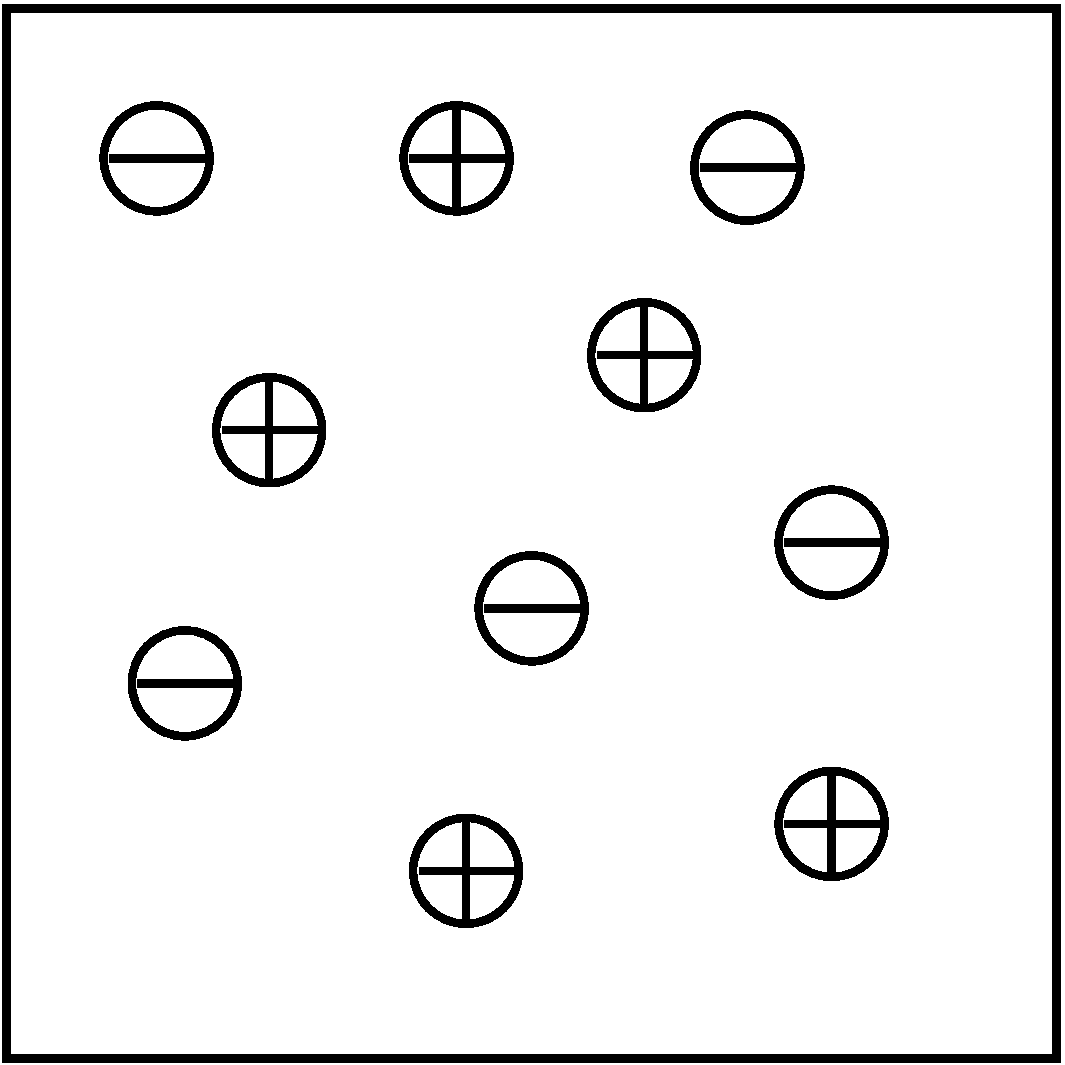
\includegraphics[width=0.4\textwidth]{figs/long-range//chargedSystem.pdf}      
%   \end{figure}
% \end{frame}
 

\begin{frame} {Electrostatic interaction}
  \vfill Electrostatic interaction between two charges
  $$\bluec{
    U_{\textrm{ele}}(\v r_{ij}) = \frac1{4\pi\varepsilon}\frac{q_i q_j}{\vert \v r_{ij}\vert}}
  $$
  \vfill
  The electrostatic energy of a periodic system is \vfill
  \begin{equation*}\bluec{
    U_{\textrm{ele}} = \frac12 \sum^\ast_{n}\sum_{i,j}\frac{q_i q_j}{\vert \v r_{ij} + \v n\vert}}
  \end{equation*}\vfill
  $\v r_{ij} = \v r_i - \v r_j$ and $\v n = n_1 \v a_1 + n_2 \v a_2 +
  n_3 \v a_3$ is the lattice in real space and the $\v a_\alpha, \
  \alpha=1,2,3$, are box vectors. \vfill
  Important applications: \redc{hydrogen bond in water}, \redc{ionic solutions},
  \redc{protein folding}...  \vfill
\end{frame}

\begin{frame}[label=Ewald]
  \frametitle{Ewald summation} Ewald summation (1921) splits the
  energy into three parts
  \bluec{
  \begin {align*}
    U_{\textrm{ele}} &=  U_{\textrm{dir}} + U_{\textrm{rec}}+ U_{\textrm{corr}}\\
    U_{\textrm{dir}} & = \frac12 \sum^{\ast}_{\v n}
    \sum_{i,j = 1}^{N} \frac{q_iq_j\, \redc{\textrm{erfc}(\beta \vert\v{r}_{ij} + \v{n}\vert)}}
    {\vert\v{r}_{ij} + \v{n}\vert} \\ \label{Erec-ewald}
    U_{\textrm{rec}} & = \frac1{2\pi V} \sum_{\v m \neq 0}
    \frac{\redc{\exp(-\pi^2\v m^2 / \beta^2)}}{\v m^2} S(\v m) S(-\v m) \\
    U_{\textrm{corr}}& = -\frac\beta{\sqrt \pi} \sum_{i=1}^N q_i^2
  \end {align*}}
  \vfill
  \hfill
  \hyperlink{key-idea-spme}{\beamerreturnbutton{To SPME}}
\end{frame}

\begin{frame}
  \frametitle{Ewald summation is $\mathcal O(N^{3/2})$} 
  The structure factor $S(\v m)$ is
  defined by \bluec{
    \begin{equation*}\label{sm1}
      S(\v m) = \sum_{j=1}^N q_j \exp (2 \pi i \v m \cdot \v r_j),
    \end{equation*}}
  Due to the fast convergence of 
  $\redc{\textrm{erfc}(\beta \vert\v{r}_{ij} + \v{n}\vert)}$ and 
  $\redc{\exp(-\pi^2\v m^2 / \beta^2)}$, the Ewald summation can be cut-offed.
  \vfill
  \bluec{\textit{J.W. Perram, H.G. Petersen and S.W. De Leeuw (1988)}}
  proved the optimized computational cost of Ewald summation is 
  \begin{align*}
    \begin{tabular}[t]{c}
      \redc{$\mathcal O(N^{3/2})$}\\
      {direct}
    \end{tabular}
    +
    \begin{tabular}[t]{c}
      \redc{$\mathcal O(N^{3/2})$}\\
      {reciprocal}
    \end{tabular}
    =
    \begin{tabular}[t]{c}
      \redc{$\mathcal O(N^{3/2})$}\\
      {total cost}
    \end{tabular}
  \end{align*} 
 \vfill 
\end{frame}



\begin{frame}
  \frametitle{Some popular $\mathcal O(N\log N)$ algorithms}
  \vfill
  \begin{itemize}
    \item The particle mesh Ewald method (\redc{PME})\\
      \bluec{\textit{T. Darden, D. York and L. Pedersen (1993)}}\\
      Times of citation: \redc{3,792} 
      \vfill
    \item The smooth particle mesh Ewald method (\redc{SPME})\\
      \bluec{\textit{U. Essmann, L. Perera, M.L. Berkowitz et al. (1995)}}\\
      Times of citation: \redc{3,162}
  \end{itemize}
  \vfill
  Times of citation is from \texttt{www.isiknowledge.com}.
  \vfill
\end{frame}


\begin{frame}[label=key-idea-spme]
  \frametitle{The key idea of SPME} 
  \vfill
  The term
  \bluec{$$ \exp (2 \pi i \v m \cdot \v r_j) $$}
  in factor $S(\v m)$ is first calculated on a grid. If we want to
  measure this value at any other position, it is interpolated by
  known values on the neighboring grid points. 
  \begin{itemize}
  \item PME uses \redc{Lagrangian interpolation}
  \item SPME uses  \redc{cardinal B-spline interpolation}.
  \end{itemize}
  
  \vfill
  The computational cost is 
  \begin{align*}
    \begin{tabular}[t]{c}
      \redc{$\mathcal O(N)$}\\
      {direct}
    \end{tabular}
    +
    \begin{tabular}[t]{c}
      \redc{$\mathcal O(N)$}\\
      {interpolation}
    \end{tabular}
    +
    \begin{tabular}[t]{c}
      \redc{$\mathcal O(N\log N)$}\\
      {FFTs}
    \end{tabular}
    =
    \begin{tabular}[t]{c}
      \redc{$\mathcal O(N\log N)$}\\
      {total cost}
    \end{tabular}
  \end{align*} 
 \vfill \hfill
  \hyperlink{Ewald}{\beamergotobutton{To Ewald summation}}
\end{frame}


\begin{frame}
  \frametitle{Parameters in SPME}
  \vfill
  To use SPME method, one should provide the following parameters.
  \vfill
  \begin{itemize}
    \item \redc{$\beta$} \quad The same as $\beta$ in Ewald summation.
    \item \redc{$r_c$} \quad The cut off used in the neighbor/cell list searching method for direct part.
    \item \redc{$n$} \quad The order of cardinal B-splines.
    \item \redc{$\v K$} \quad The number of grid points used to discrete the space.
  \end{itemize}
  \vfill An arbitrary choice may lead to \redc{totally wrong
    results}. \vfill
\end{frame}


\begin{frame}
  \frametitle{Two branches of SPME force} 
  \vfill
  The general formula of calculating force from energy of a particle system is 
  \bluec{$$ \v F_i = - \nabla_{\v r_i} U $$}
  There are two possible ways of calculating forces in the charged system.
  \vfill
  \begin{itemize}
  \item \redc{ik differentiation} \newline Derivative -- interpolate
  \item \redc{analytical differentiation} \newline Interpolate -- derivative
  \end{itemize}
  \vfill
  Which method is better was an \redc{open question}.
  \vfill
\end{frame}


\begin{frame}[label=expense-esti]
  \frametitle{Expense estimate}
  The expense estimate is trivial
  \vfill
  \begin{itemize}
  \item Direct part \quad \bluec{$T^{\textrm{dir}} \approx C_d\redc{r_c}^3$} \vfill
  \item Reciprocal part \vfill
    \begin{itemize}
    \item ik differentiation \newline
      \bluec{$$
      T^{\textrm{rec}}_{\textrm{ik}}
      \approx C_{\textrm{ik}} N\redc{n}^3 + 4\, C_f  \redc{K_1K_2K_3} \log (\redc{K_1K_2K_3}) 
      $$}
    \item analytical differentiation\newline
      \bluec{$$
      T^{\textrm{rec}}_{\textrm{ana}}
      \approx C_{\textrm{ana}} N\redc{n}^3 + 2\, C_f  \redc{K_1K_2K_3} \log (\redc{K_1K_2K_3}).
      $$}
    \end{itemize}
  \end{itemize}
  \vfill \hfill
  \hyperlink{figure-fix-mesh}{\beamerreturnbutton{To error plot}}
\end{frame}


\begin{frame}
  \frametitle{The definition of error}\vfill
  Before we develop the error estimation for SPME, we should define the word 
  ``error'' properly. 
  \vfill
We adopt the root mean square (RMS) force error that is widely used
in this field: $$ \bluec{\mathcal E(r_c, \v K, n, \beta) = \sqrt{\langle(\v
  F^{\textrm{exact}} - \v F^{\textrm{{approx}}})^2\rangle} }$$
$\v F^{\d {exact}}$ and $\v F^{\d {approx}}$ denote the exact
electrostatic interaction and SPME calculated force, respectively.
\vfill
\end{frame}


\begin{frame}
  \frametitle{The definition of error}\vfill
  The RMS force error is not easy to calculate in practice. 
  We consider the RMS force error of direct part and reciprocal part.
  \bluec{
    \begin{align*}
      \mathcal E^{\textrm{dir}}(r_c, \beta) =& 
      \sqrt{\langle(\v F^{\textrm{{approx}}}_{\textrm{{dir}}} - \v F^{\textrm{exact}}_{\textrm{dir}})^2\rangle} \\
      \mathcal E^{\textrm{rec}}(\v K, n, \beta) = &
      \sqrt{\langle(\v F^{\textrm{{approx}}}_{\textrm{{rec}}} - \v F^{\textrm{exact}}_{\textrm{rec}})^2\rangle}
    \end{align*}}
  where $\v F^{\textrm{exact}}_{\textrm{dir}}$ and
  $\v F^{\textrm{exact}}_{\textrm{rec}}$ are direct and reciprocal part of
  Ewald summation \redc{without} cut-off. \bluec{ $\v F^{\textrm{exact}} =
    \v F^{\textrm{exact}}_{\textrm{dir}} + \v F^{\textrm{exact}}_{\textrm{rec}}
    $}.
  \vfill
  $\v F^{\textrm{approx}}_{\textrm{dir}}$ and $\v
  F^{\textrm{approx}}_{\textrm{rec}}$ are direct and reciprocal part of
  SPME force. \bluec{$\v F^{\textrm{approx}} =
    \v F^{\textrm{approx}}_{\textrm{dir}} + \v F^{\textrm{approx}}_{\textrm{rec}}
    $}.
  \vfill
  In most cases, we have \redc{
  $\frac12(\mathcal E^{\textrm{dir}} + \mathcal E^{\textrm{rec}}) \leq
  \mathcal E \leq (\mathcal E^{\textrm{dir}} +
  \mathcal E^{\textrm{rec}})$}
\end{frame}


\begin{frame}
  \frametitle{The definition of error}\vfill
  $\mathcal E^{\textrm{dir}}$ is actually the same as cut-off Ewald
  summation, which was given by \bluec{J. Kolafa and
    J.W. Perram. (1992)}.
  \vfill
  The calculation of $\mathcal E^{\textrm{rec}}(\v K, n, \beta)$ is not straight forward.
  Alternatively, we define 
  $$ \bluec{\mathcal E^{\textrm{rec}}(\v K, n, \beta) \approx \sqrt{\langle(\v
  F_{\textrm{rec}}^{\textrm{{approx}}} - \v
  F_{\textrm{rec}}^{\textrm{{cut}}})^2\rangle} }$$
where $\v
F_{\textrm{rec}}^{\textrm{{cut}}}$ is the force derived by the Ewald
summation using the same set of parameters as the SPME method. The reason is \redc{
$ \sqrt{\langle(\v
  F_{\textrm{rec}}^{\textrm{{approx}}} - \v
  F_{\textrm{rec}}^{\textrm{{cut}}})^2\rangle} $ is comparatively much
larger than $ \sqrt{\langle(\v F_{\textrm{rec}}^{\textrm{cut}} - \v
  F_{\textrm{rec}}^{\textrm{exact}})^2\rangle} $.} \vfill
\end{frame}


\begin{frame}[label=figure-fix-order]
  \frametitle{Numerical result of the error estimate. Fix $r_c$ and order $n=6$}
  \begin{figure}
  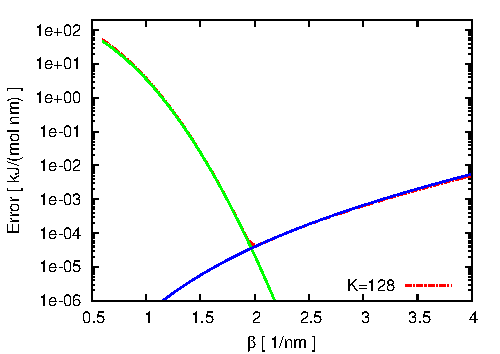
\includegraphics[width=0.8\textwidth]{figs/long-range//bspline-order6.pdf}
  \caption{The actual and estimated error of ik differentiation as a
    function of $\beta$.   } 
\end{figure}
\vfill\hfill
\hyperlink{tune-assumption}{\beamerreturnbutton{To assumption}}
\end{frame}


\begin{frame}[label=figure-fix-mesh]
  \frametitle{Numerical result of the error estimate. Fix $r_c$ and grid $\v K = (32, 32, 32)$}
  \begin{figure}
    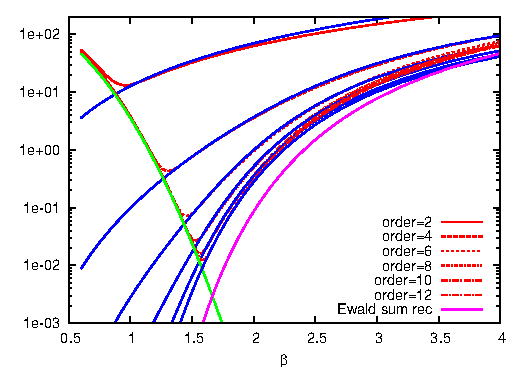
\includegraphics[width=0.8\textwidth]{figs/long-range//bspline-mesh32.pdf}
    \caption{The actual and estimated error of ik differentiation as a
      function of $\beta$. }
  \end{figure} \hfill
  \hyperlink{expense-esti}{\beamergotobutton{To expanse}}
\end{frame}

\begin{frame}{Numerical result of the error estimate. TIP3P water system}
  \begin{figure}
    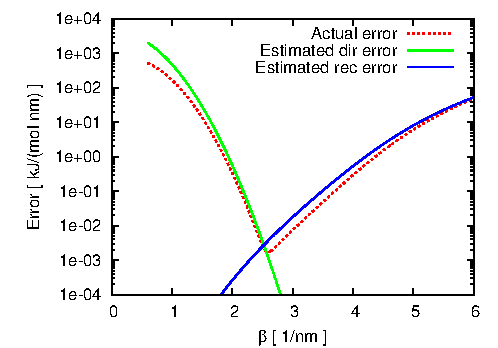
\includegraphics[width=0.8\textwidth]{figs/long-range//tip3p.pdf}
  \end{figure} \hfill
\end{frame}


\begin{frame}
  \frametitle{Parameter tuning algorithm} 
  The parameter tuning is a constrained optimization problem \bluec{
  \begin{align*} 
    \min\quad &  T (r_c, \v K, n, \beta),\\
    \textrm{\textbf{s.t.}}\quad & \mathcal E (r_c, \v K, n, \beta) = \mathcal E^\ast
  \end{align*}}
  $n = 2, 4, 6, 8$ and $\v K = (K_1, K_2, K_3)$ discrete ones. To
  ensure a high performance of the FFT, $K_\alpha$ should be able to
  decompose into small prime numbers, such as 2, 3, 5 and 7.
\end{frame}

\begin{frame}[label=tune-assumption]
  \frametitle{Splitting the original problem} Fixing $\beta$ to
  \redc{$\beta_0$}, the original problem can be decomposed into two
  \redc{independent} problems.\bluec{
  \begin{align*}
    \min\quad & 
    T^{\textrm{dir}} (r_c, \beta_0), \\* 
    \textrm{\textbf{s.t.}}\quad & 
    \mathcal E^{\textrm{dir}} (r_c, \beta_0) = \mathcal E^\ast_{\textrm{dir}},
  \end{align*}}
  \vskip -1.2cm\bluec{
  \begin{align*}
    \min\quad & 
    T^{\textrm{rec}} (\v K, n, \beta_0), \\* 
    \textrm{\textbf{s.t.}}\quad & 
    \mathcal E^{\textrm{rec}} (\v K, n, \beta_0) = \mathcal E^\ast_{\textrm{rec}},
  \end{align*}}
  Actually, it is not easy to give a set of $(\beta_0,
  \mathcal E^\ast_{\textrm{dir}}, \mathcal E^\ast_{\textrm{rec}})$
  such that the solution of the split problem is the same as the
  original problem. We assume\redc{
  $$\mathcal E^\ast_{\textrm{dir}} = \mathcal E^\ast_{\textrm{rec}} =
  \frac12\, \mathcal E^\ast$$}
\vfill\hfill
\hyperlink{figure-fix-order}{\beamergotobutton{To error}}
\end{frame}


\begin{frame}
  \frametitle{Solving split problem I} \vfill
  The direct part is reduced to a nonlinear equation
  \begin{equation*}\bluec{
    \mathcal E^{\textrm{dir}} (r_c, \beta_0) = \frac12\, \mathcal E^\ast}
  \end{equation*}
  which can be easily solved by the \redc{bisection method}.
  \vfill
\end{frame}


\begin{frame}
  \frametitle{Solving split problem II} 
  The reciprocal part is
   \bluec{
  \begin{align*}
    \min\quad & T^{\textrm{rec}} (\v K, n, \beta_0), \\* 
    \textrm{\textbf{s.t.}}\quad & \mathcal E^{\textrm{rec}} (\v K, n,
    \beta_0) = \frac12\, \mathcal E^\ast.
  \end{align*}} 
Fortunately, we only consider a finite set of $n$, that is \redc{2, 4,
  6 and 8}. Now fix $n$ to a certain number and solve the equation
with respect to $\v K$ by the \redc{bisection method}. Among the four
resulting pairs of $n$ and $\v K$, we choose the one that minimize
$T^{\textrm{rec}}$.
\end{frame}

\begin{frame}
  \frametitle{Find out the optimal $\beta$ }
  \vfill
  Now given a certain $\beta_0$, we can find a set of parameters
  $(r_{c}(\beta_0), \v K(\beta_0), n (\beta_0))$ that optimize the
  split problem. 
  \vfill
  Consider the mapping 
  \bluec{$$T =  T(r_{c}(\beta), \v K(\beta), n (\beta), \beta)$$}
  Since this mapping is not smooth (because $\v K$ and $n$ are
  discrete numbers), we use \redc{0.618 searching method} to find out
  the solution.  \vfill
\end{frame}


\begin{frame}
  \frametitle{Optimal parameters of ik differentiation}
\begin{table}
  \centering
  \begin{tabular*}{0.6\textwidth}{@{\extracolsep{\fill}}ccccc}
  % \begin{tabular}{r|cccc}
    $N$    & $r_c$ [$\textsf{nm}$] & $\v K$ & $n$& $\beta$ [$\textsf{nm}^{-1}$]\\ \hline
    $8^3$ & 2.980 & $40^3$ & 6 & 1.202 \\
    $10^3$ & 3.005 & $50^3$ & 6 & 1.191  \\
    $15^3$ & 3.089 & $72^3$ & 6 & 1.154  \\
    $20^3$ & 3.019 & $100^3$ & 6 & 1.182  \\
    $25^3$ & 2.940 & $128^3$ & 6 & 1.215 \\
    $30^3$ & 3.170 & $140^3$ & 6 & 1.128  \\
    $40^3$ & 3.170 & $189^3$ & 6 & 1.128  
  \end{tabular*}
  \caption{
    Optimal parameters of ik differentiation. 
    The target precision is $\mathcal E^\ast=10^{-3}\,\textsf{KJ/(mol\,nm)}$.
  }
\end{table}
\end{frame}


\begin{frame}
  \frametitle{Accuracy of ik differentiation}
\begin{table}
  \centering
  \begin{tabular*}{0.95\textwidth}{@{\extracolsep{\fill}}cccc}
    $N$ & $\mathcal E\,[\textsf{KJ/(mol\,nm)}]$ & $\mathcal E_{\textrm{dir}}\,[\textsf{KJ/(mol\,nm)}]$ & $\mathcal E_{\textrm{rec}}\,[\textsf{KJ/(mol\,nm)}]$ \\ \hline
    $8^3$ & $6.47\times10^{-4}$ & $4.31\times10^{-4}$ & $4.95\times10^{-4}$   \\
    $10^3$ & $6.41\times10^{-4}$ & $4.39\times10^{-4}$ & $4.63\times10^{-4}$   \\
    $15^3$ & $6.94\times10^{-4}$ & $4.79\times10^{-4}$ & $4.85\times10^{-4}$   \\
    $20^3$ & $6.55\times10^{-4}$ & $4.72\times10^{-4}$ & $4.39\times10^{-4}$   \\
    $25^3$ & $6.54\times10^{-4}$ & $4.66\times10^{-4}$ & $4.56\times10^{-4}$   \\
    $30^3$ & $6.67\times10^{-4}$ & $4.37\times10^{-4}$ & $4.97\times10^{-4}$   \\
    $40^3$ & $6.43\times10^{-4}$ & $4.37\times10^{-4}$ & $4.58\times10^{-4}$   
  \end{tabular*}
  \caption{
    Accuracy of ik differentiation. 
    The target precision is $\mathcal E^\ast=10^{-3}\,\textsf{KJ/(mol\,nm)}$.
  }
\end{table}
\end{frame}

\begin{frame}
  \frametitle{Computational expense of ik differentiation}
\begin{figure}
  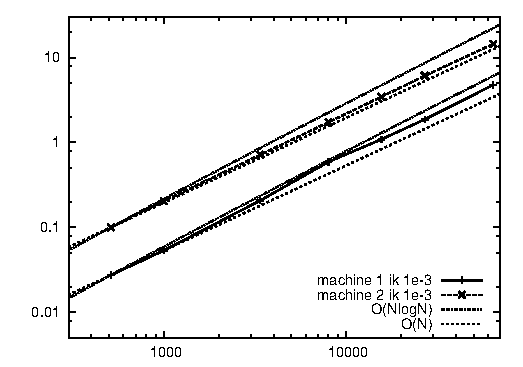
\includegraphics[width=0.8\textwidth]{figs/long-range//both-time-1e-3.pdf}
  \caption{Computational cost of ik differentiated SPME method as a
    function of particle number. The target precision is
    $\mathcal E^\ast=10^{-3}\,\textsf{KJ/(mol\,nm)}$.}
\end{figure}
\end{frame}

\begin{frame}
  \frametitle{Comparison between ik differentiation and analytical differentiation. Computational expense}
\begin{table}
  \centering
  \begin{tabular}{r|r|r}
    $N$    & ik & ana \\ \hline
    $8^3$ & $0.101$  &$0.117$ \\
    $10^3$ & $0.204$ &$0.232$ \\
    $15^3$ & $0.700$ &$0.805$ \\
    $20^3$ & $1.730$ &$1.970$  \\
    $25^3$ & $3.420$ &$3.930$ \\
    $30^3$ & $6.160$ &$6.980$  \\
    $40^3$ & $15.300$  &$15.790$ 
  \end{tabular}
  \caption{
    Comparison of computational cost between ik-differentiation and analytical differentiation.
  }
\end{table}
\end{frame}


\begin{frame}
  \frametitle{Comparison between ik differentiation and analytical differentiation. Parameters}
\begin{table}
  \centering
  \begin{tabular}{r|c|c|c|c}
    $N$    & $r_c$ & $\v K$ & $n$& $\beta$\\ \hline
    $8^3$ & 2.980 & $40^3$ & 6 & 1.202 \\
    $10^3$ & 3.005 & $50^3$ & 6 & 1.191  \\
    $15^3$ & 3.089 & $72^3$ & 6 & 1.154  \\
    $20^3$ & 3.019 & $100^3$ & 6 & 1.182  \\
    $25^3$ & 2.940 & $128^3$ & 6 & 1.215 \\
    $30^3$ & 3.170 & $140^3$ & 6 & 1.128  \\
    $40^3$ & 3.170 & $189^3$ & 6 & 1.128  
  \end{tabular}
  \hfill
  \begin{tabular}{c|c|c|c}
     $r_c$ & $\v K$ & $n$& $\beta$  \\ \hline
     3.115 & $48^3$ & 6 & 1.146  \\
     3.073 & $60^3$ & 6 & 1.166  \\
     3.089 & $90^3$ & 6 & 1.154  \\
     2.950 & $125^3$ & 6 & 1.215  \\
     2.901 & $162^3$ & 6 & 1.235  \\
     2.940 & $189^3$ & 6 & 1.215  \\
     3.267 & $224^3$ & 6 & 1.095 
  \end{tabular}
  \caption{
    Comparison of parameters between ik differentiation and analytical differentiation.
  }
\end{table}
\end{frame}


\begin{frame}
  \frametitle{Parameter tuning according to the reference system}
\begin{table}
  \centering
  \begin{tabular}{r|c|c|c|c|r}
    $N$    &  $\v K$ & $\mathcal E$ & $\mathcal E_{\textrm{dir}}$ & $\mathcal E_{\textrm{rec}}$ & $T$ (s) \\ \hline
$8^3$ & $40^3$ &  $5.97\times10^{-4}$ & $4.79\times10^{-4}$ & $3.70\times10^{-4}$ & $0.104$  \\
$10^3$ & $48^3$ &  $6.91\times10^{-4}$ & $4.79\times10^{-4}$ & $4.85\times10^{-4}$ & $0.206$  \\
$15^3$ & $72^3$ &  $6.94\times10^{-4}$ & $4.79\times10^{-4}$ & $4.85\times10^{-4}$ & $0.715$  \\
$20^3$ & $96^3$ &  $6.95\times10^{-4}$ & $4.79\times10^{-4}$ & $4.85\times10^{-4}$ & $1.670$  \\
$25^3$ & $120^3$ &  $6.84\times10^{-4}$ & $4.79\times10^{-4}$ & $4.85\times10^{-4}$ & $3.410$  \\
$30^3$ & $144^3$ &  $6.90\times10^{-4}$ & $4.79\times10^{-4}$ & $4.85\times10^{-4}$ & $5.810$  \\
$40^3$ & $192^3$ &  $6.94\times10^{-4}$ & $4.79\times10^{-4}$ & $4.85\times10^{-4}$ & $13.790$  
  \end{tabular}
  \caption{Use $N=15^3$ as reference system. 
    Optimal $\v K$, accuracy and computational cost of ik differentiation. 
  }
\end{table}
\end{frame}

\begin{frame}
  \frametitle{Parameter tuning according to the reference system}
\begin{figure}
  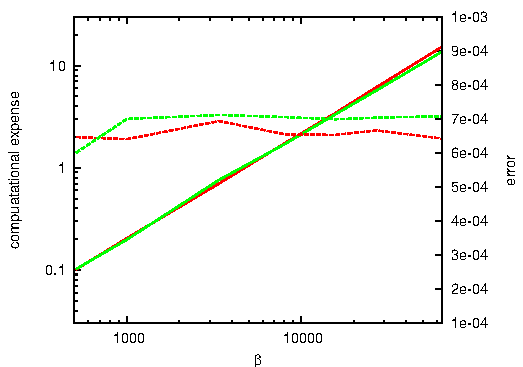
\includegraphics[width=0.8\textwidth]{figs/long-range//tune2.pdf}
  \caption{Comparison between direct tuning algorithm (red) and tuning according to the reference system (green).
  The solid lines are computational expenses and the dashed lines are errors.}
\end{figure}
\end{frame}




\begin{frame}
  \centerline{ \Huge
  Thanks! } 
\end{frame}






\end{document}
